\subsection{Experiments}\label{subsec:rupture_experiments}

In this section we provide results on various experiments we conducted in
laboratory environment to evaluate the performance of Rupture. These results
reflect Rupture's versatility when it comes to attacking different protocols and
are a good basis in order to evaluate the tool against real-world systems in
future work.

Our laboratory environment consisted of a single web page which is hosted on an
Nginx web server.\footnote[2]{The laboratory URLs used for experimentation have
been removed in the anonymized version of the paper.} This page contains digits
and a single word, which consists of 8 lowercase English letters and serves as
the secret. The first two characters of the word are known and were used in
order to bootstrap the attack. It also offers a GET URL parameter and reflects
the parameter's value in the middle of the digits in the page.

This page is the most basic scenario for a BREACH attack. It is noiseless and
the secret's alphabet is different from the rest of the page. We were also
careful to remove any repetitions of digrams in order to avoid the possibility
of compression with different parts of the page.

We deployed all Rupture modules on a single machine and used this same machine
as victim to avoid the need for injection. We also configured Rupture's
acceptable confidence level to 0.6 bytes and the secret's alphabet to all 26
lowercase English letters.

Finally, we utilized most optimizations proposed in the previous sections. We
used all uppercase English letters for the block alignment, issued 32 requests
in parallel for each character candidate in the form of a soup, and used the
divide and conquer method for computing the reflection strings.

Figure \ref{fig:rupture_performance_div_conq} shows the results of our first
experiment against the AES algorithm in GCM and CBC modes for block sizes of
128 and 256 bits.

   \begin{figure}[thpb]
      \centering
          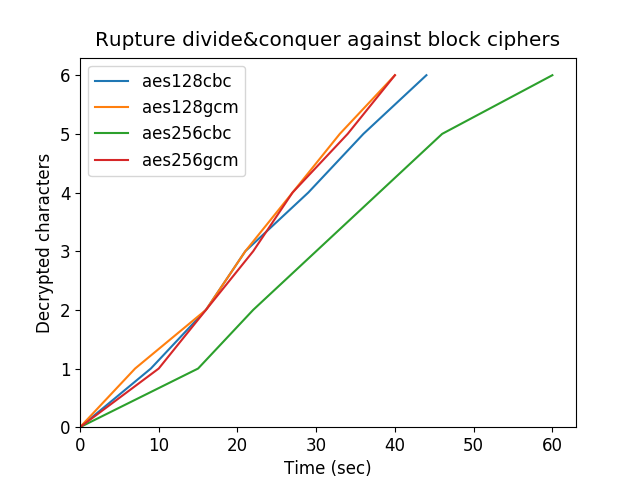
\includegraphics[width=0.48\textwidth]{experiments/rupture_performance/rupture_div_conq_performance.png}
       \caption{Rupture divide and conquer performance}
      \label{fig:rupture_performance_div_conq}
   \end{figure}

We were able to consistently decrypt all unknown characters of the word in all
cases. The total time for decrypting the 6 characters ranged from 38 seconds, in
the case of GCM mode 128-bit block size, to 48 seconds, in the case of GCM mode
256-bit block size. Therefore the average time for decrypting a single character
using the divide and conquer method was 6-8 seconds.

In our second experiment we tested the consistency of Rupture by targeting a
longer secret. This time the secret was 25 characters long and we used the
serial method for computing the reflections. The rest of the experiment
parameters were the same as previously.

Figure \ref{fig:rupture_performance_serial} shows the results of the second
experiment.

   \begin{figure}[thpb]
      \centering
          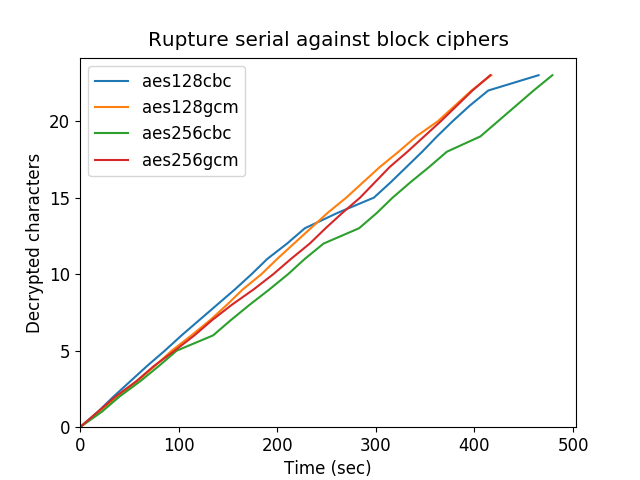
\includegraphics[width=0.48\textwidth]{experiments/rupture_performance/rupture_serial_performance.png}
      \caption{Rupture serial performance}
      \label{fig:rupture_performance_serial}
   \end{figure}

Again we were able to decrypt all unknown characters in all AES modes and block
sizes. This time the total time ranged from 416 (GCM-256) to 479 (CBC-256)
seconds. Therefore the average time for decrypting a single character using the
serial method was 18-21 seconds.
